\chapter{Simulations}\label{c:simulations}

This chapter details the attempts at reproducing micropillar tensile tests on single crystal Ni, performed by Alan Xu and Dhriti Bhattacharyya at ANSTO Sydney.

\section{Methodology}

\subsection{Experimental setup}
\label{ss:experimentalSetup}

In total, eight loading tests were carried out.
\begin{enumerate}
    \item Loading in the $\langle 1\, 0\, 0 \rangle$:
          \begin{enumerate}
              \item Two tests with a loading rate of $\SI{5}{\nano\metre\per\second}$.
              \item Two tests with a loading rate of $\SI{500}{\nano\metre\per\second}$.
          \end{enumerate}
    \item Loading in the $\langle 1\, 1\, 0 \rangle$:
          \begin{enumerate}
              \item Two tests with a loading rate of $\SI{5}{\nano\metre\per\second}$.
              \item Two tests with a loading rate of $\SI{500}{\nano\metre\per\second}$.
          \end{enumerate}
\end{enumerate}

The cross-section of the micropillars was well-known at $\SI{12}{\micro\metre} \times \SI{12}{\micro\metre}$, however the length was postulated to be $\sim \SI{30}{\micro\metre}$.

The initial dislocation configuration was not well known but was postulated to be approximately 10 dislocations per square micron. The total length of mobile dislocations influences how much plasticity we observe. Furthermore, the Frank-Reed (FR) source length was unknown. A dislocation line's yield stress is inversely proportional to its length,
\begin{align}\label{eq:yieldStress}
    \sigma_\rvar{y} & = \dfrac{\mu b}{l}\,,
\end{align}
where $\sigma_\rvar{y}$ is the yield stress, $\mu$ the shear modulus, $b =  \vec{b} $, and $l$ the dislocation line length. Both of these parameters had to be estimated and refined by running probing simulations.

The tensile tests were set up as shown in \cref{f:expSetup}. The pillars were placed under tensile load in the $x$-direction but were free to move in the $xy$-plane, which would naturally happen as dislocations exit the surface and create slip steps.
\begin{figure}
    \centering
    \begin{subfigure}[t]{0.45\linewidth}
        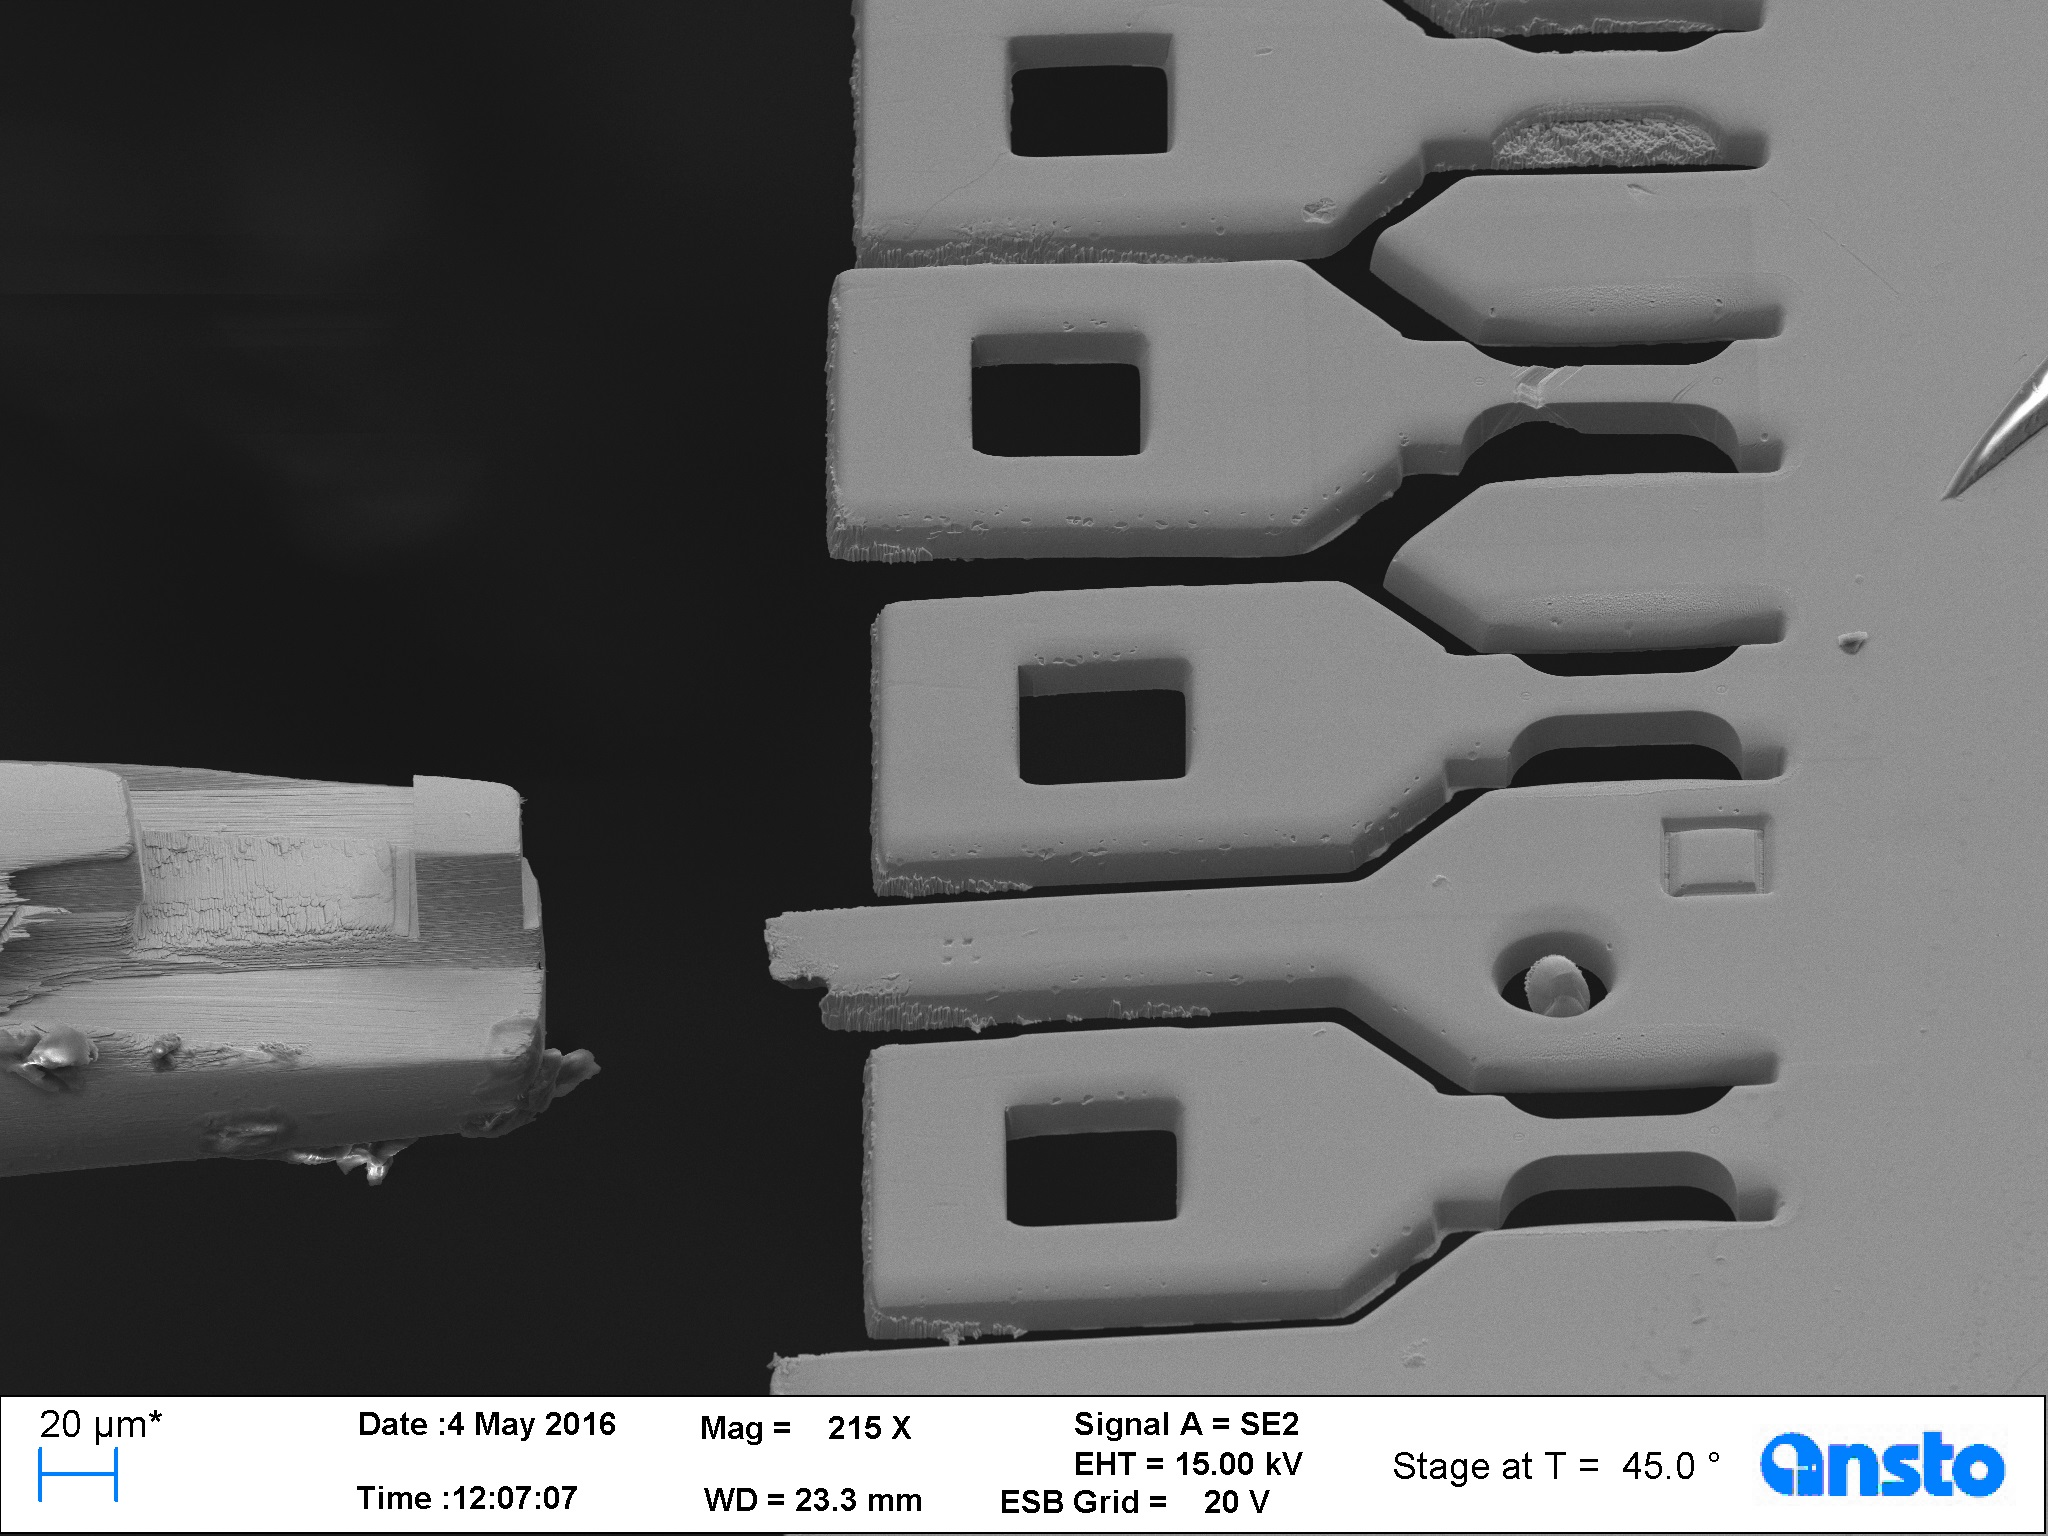
\includegraphics[width=\linewidth]{../data/Ni024.jpg}
        \caption[Stage for micropillar tensile tests.]{Stage for micropillar tensile tests. Ensemble setup, pillars are pulled from the square hole. They are allowed to freely move in the $yz$-plane.}
    \end{subfigure}
    ~
    \begin{subfigure}[t]{0.45\linewidth}
        \centering
        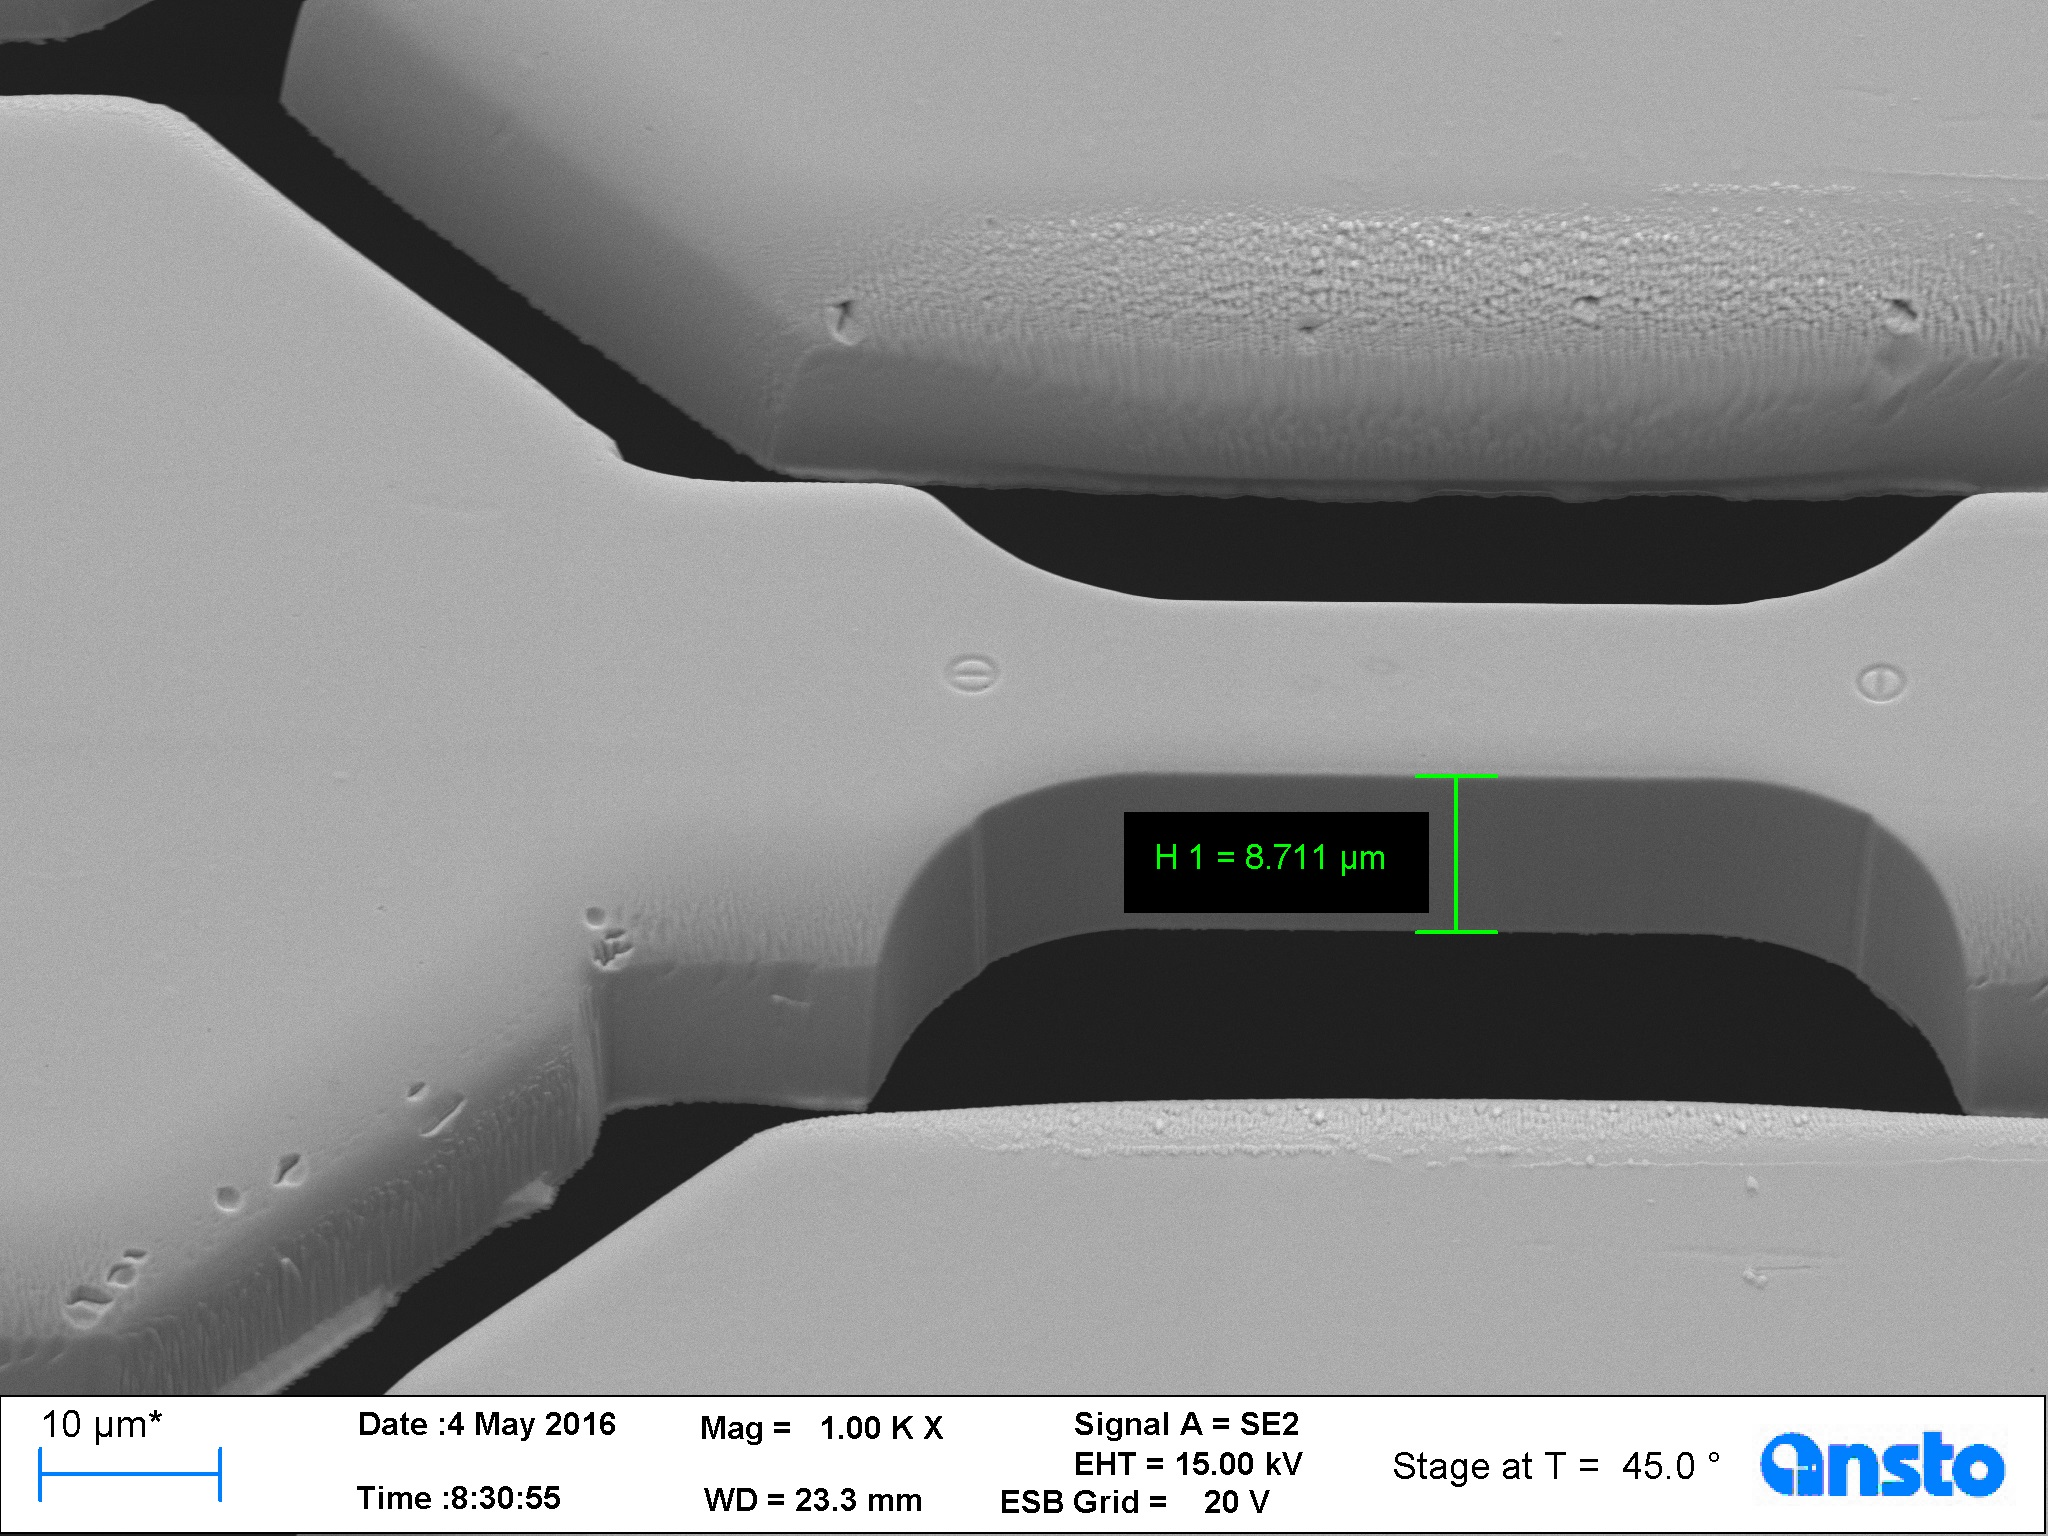
\includegraphics[width=\linewidth]{../data/Ni000.jpg}
        \caption[Close up of the initial state of a single pillar.]{Close up of the initial state of a single pillar. Camera is at $\SI{45}{\degree}$, square cross-section measures $\SI{12}{\micro\metre}$ per side, length is $\sim \SI{30}{\micro\metre}$.}
    \end{subfigure}
    \caption{Experimental stage for tensile tests on Ni micropillars.}
    \label{f:expSetup}
\end{figure}
The load was applied until the pillars failed by necking, as shown in \cref{f:necking}.
\begin{figure}
    \centering
    \begin{subfigure}[t]{0.3\linewidth}
        \centering
        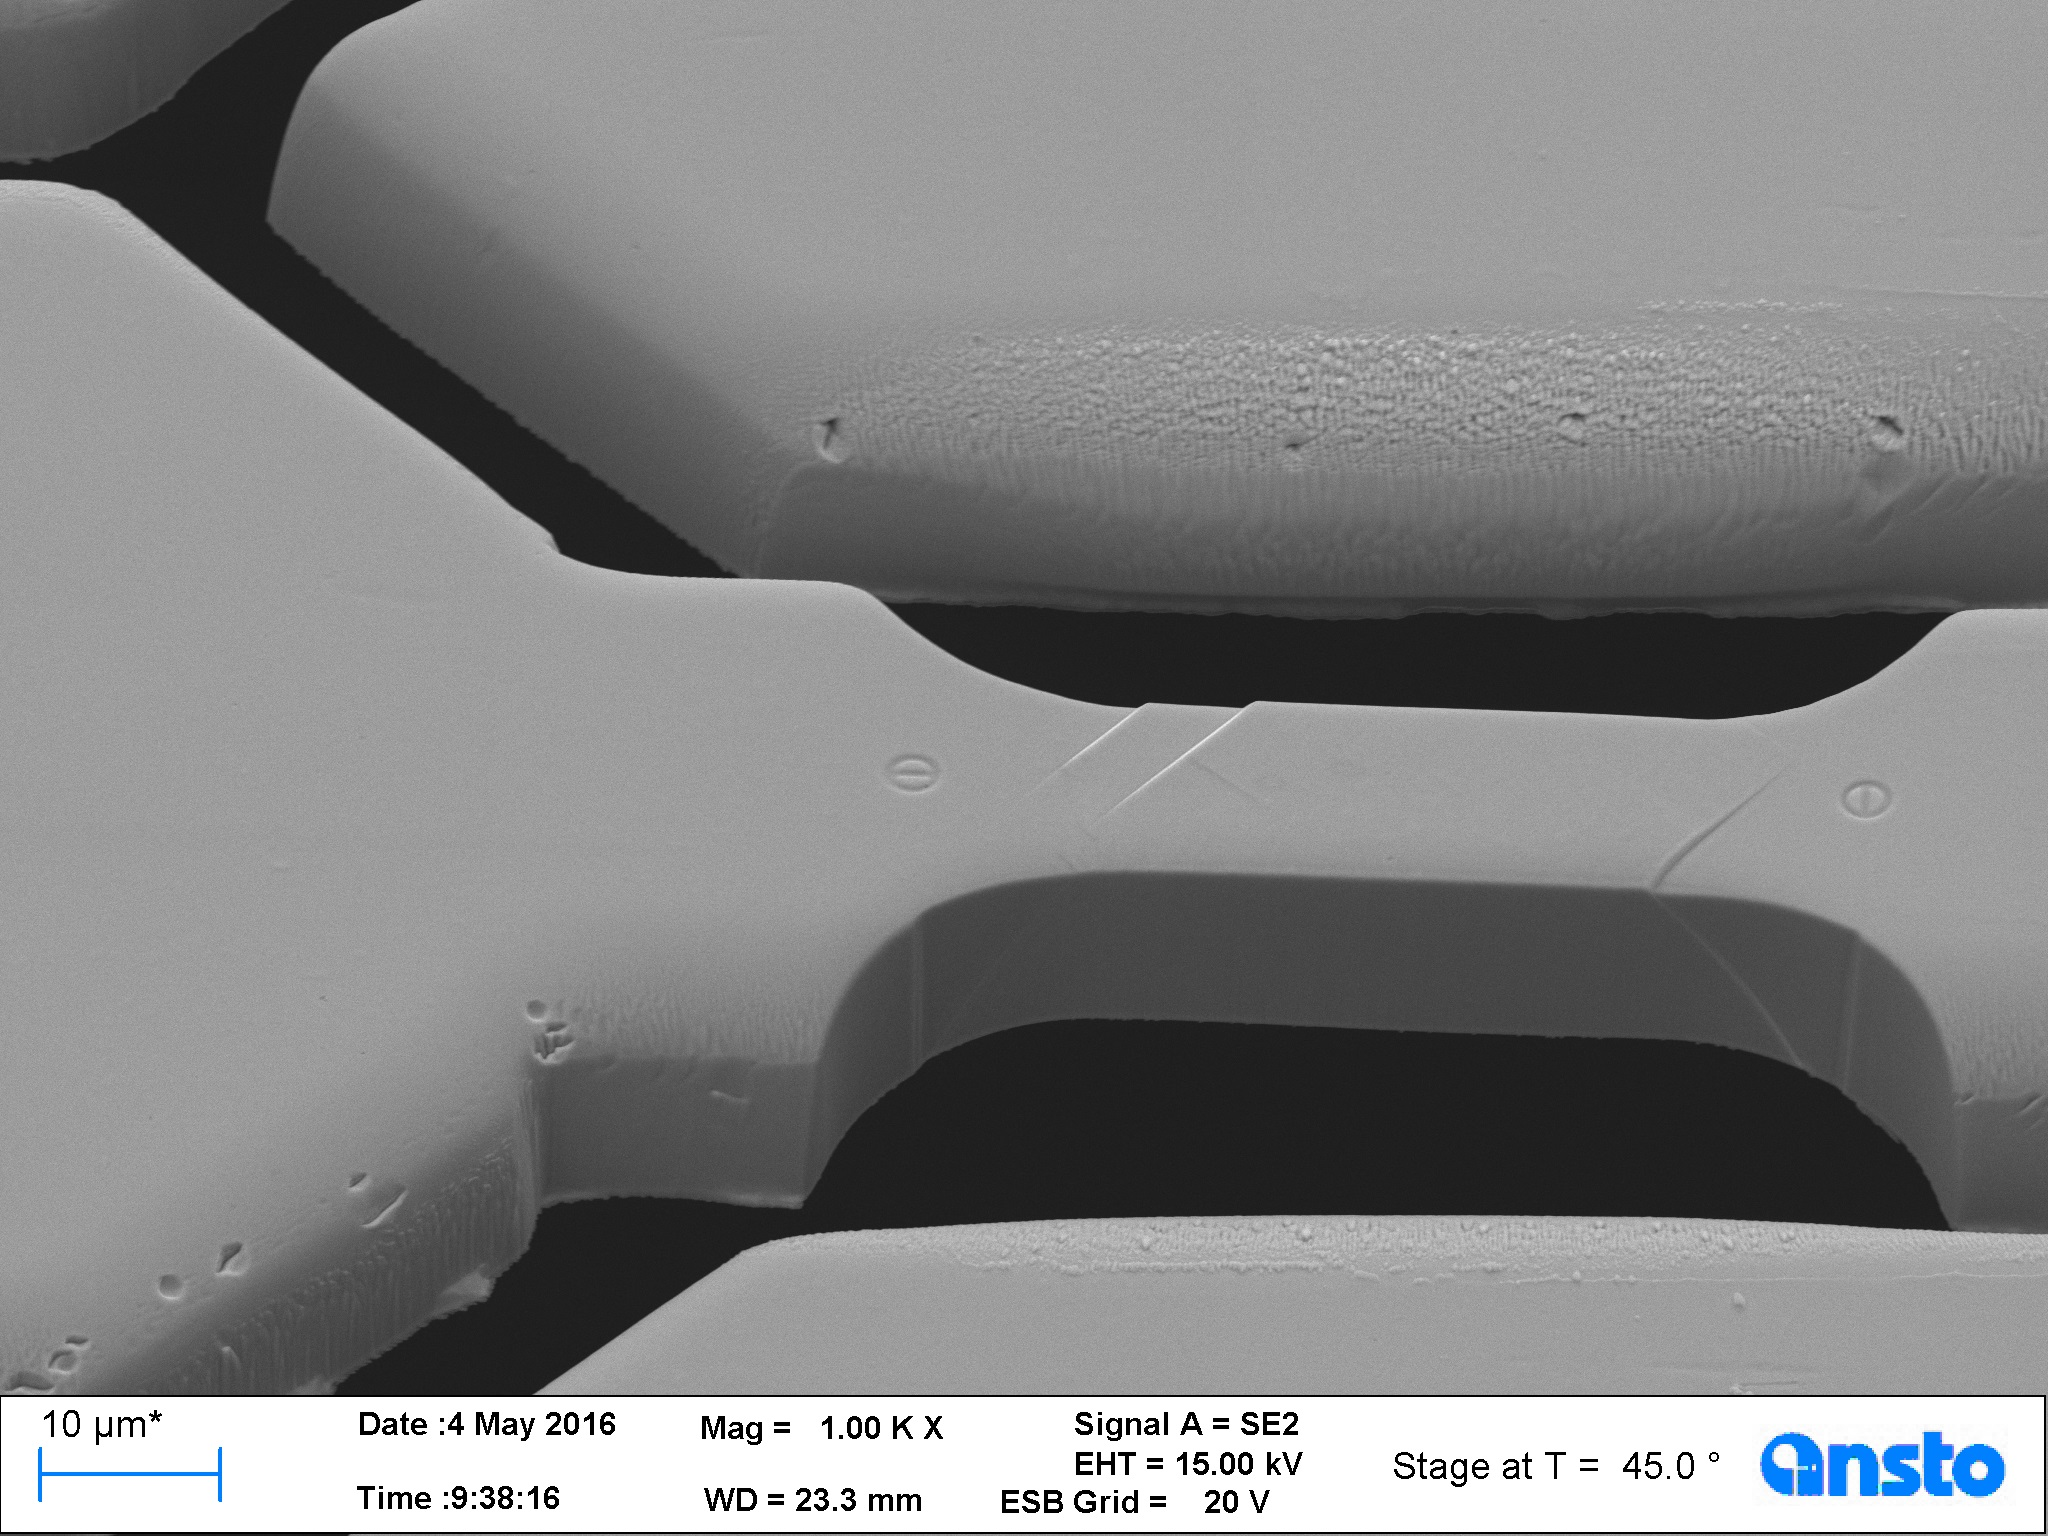
\includegraphics[width=\linewidth]{../data/Ni016.jpg}
    \end{subfigure}
    ~
    \begin{subfigure}[t]{0.3\linewidth}
        \centering
        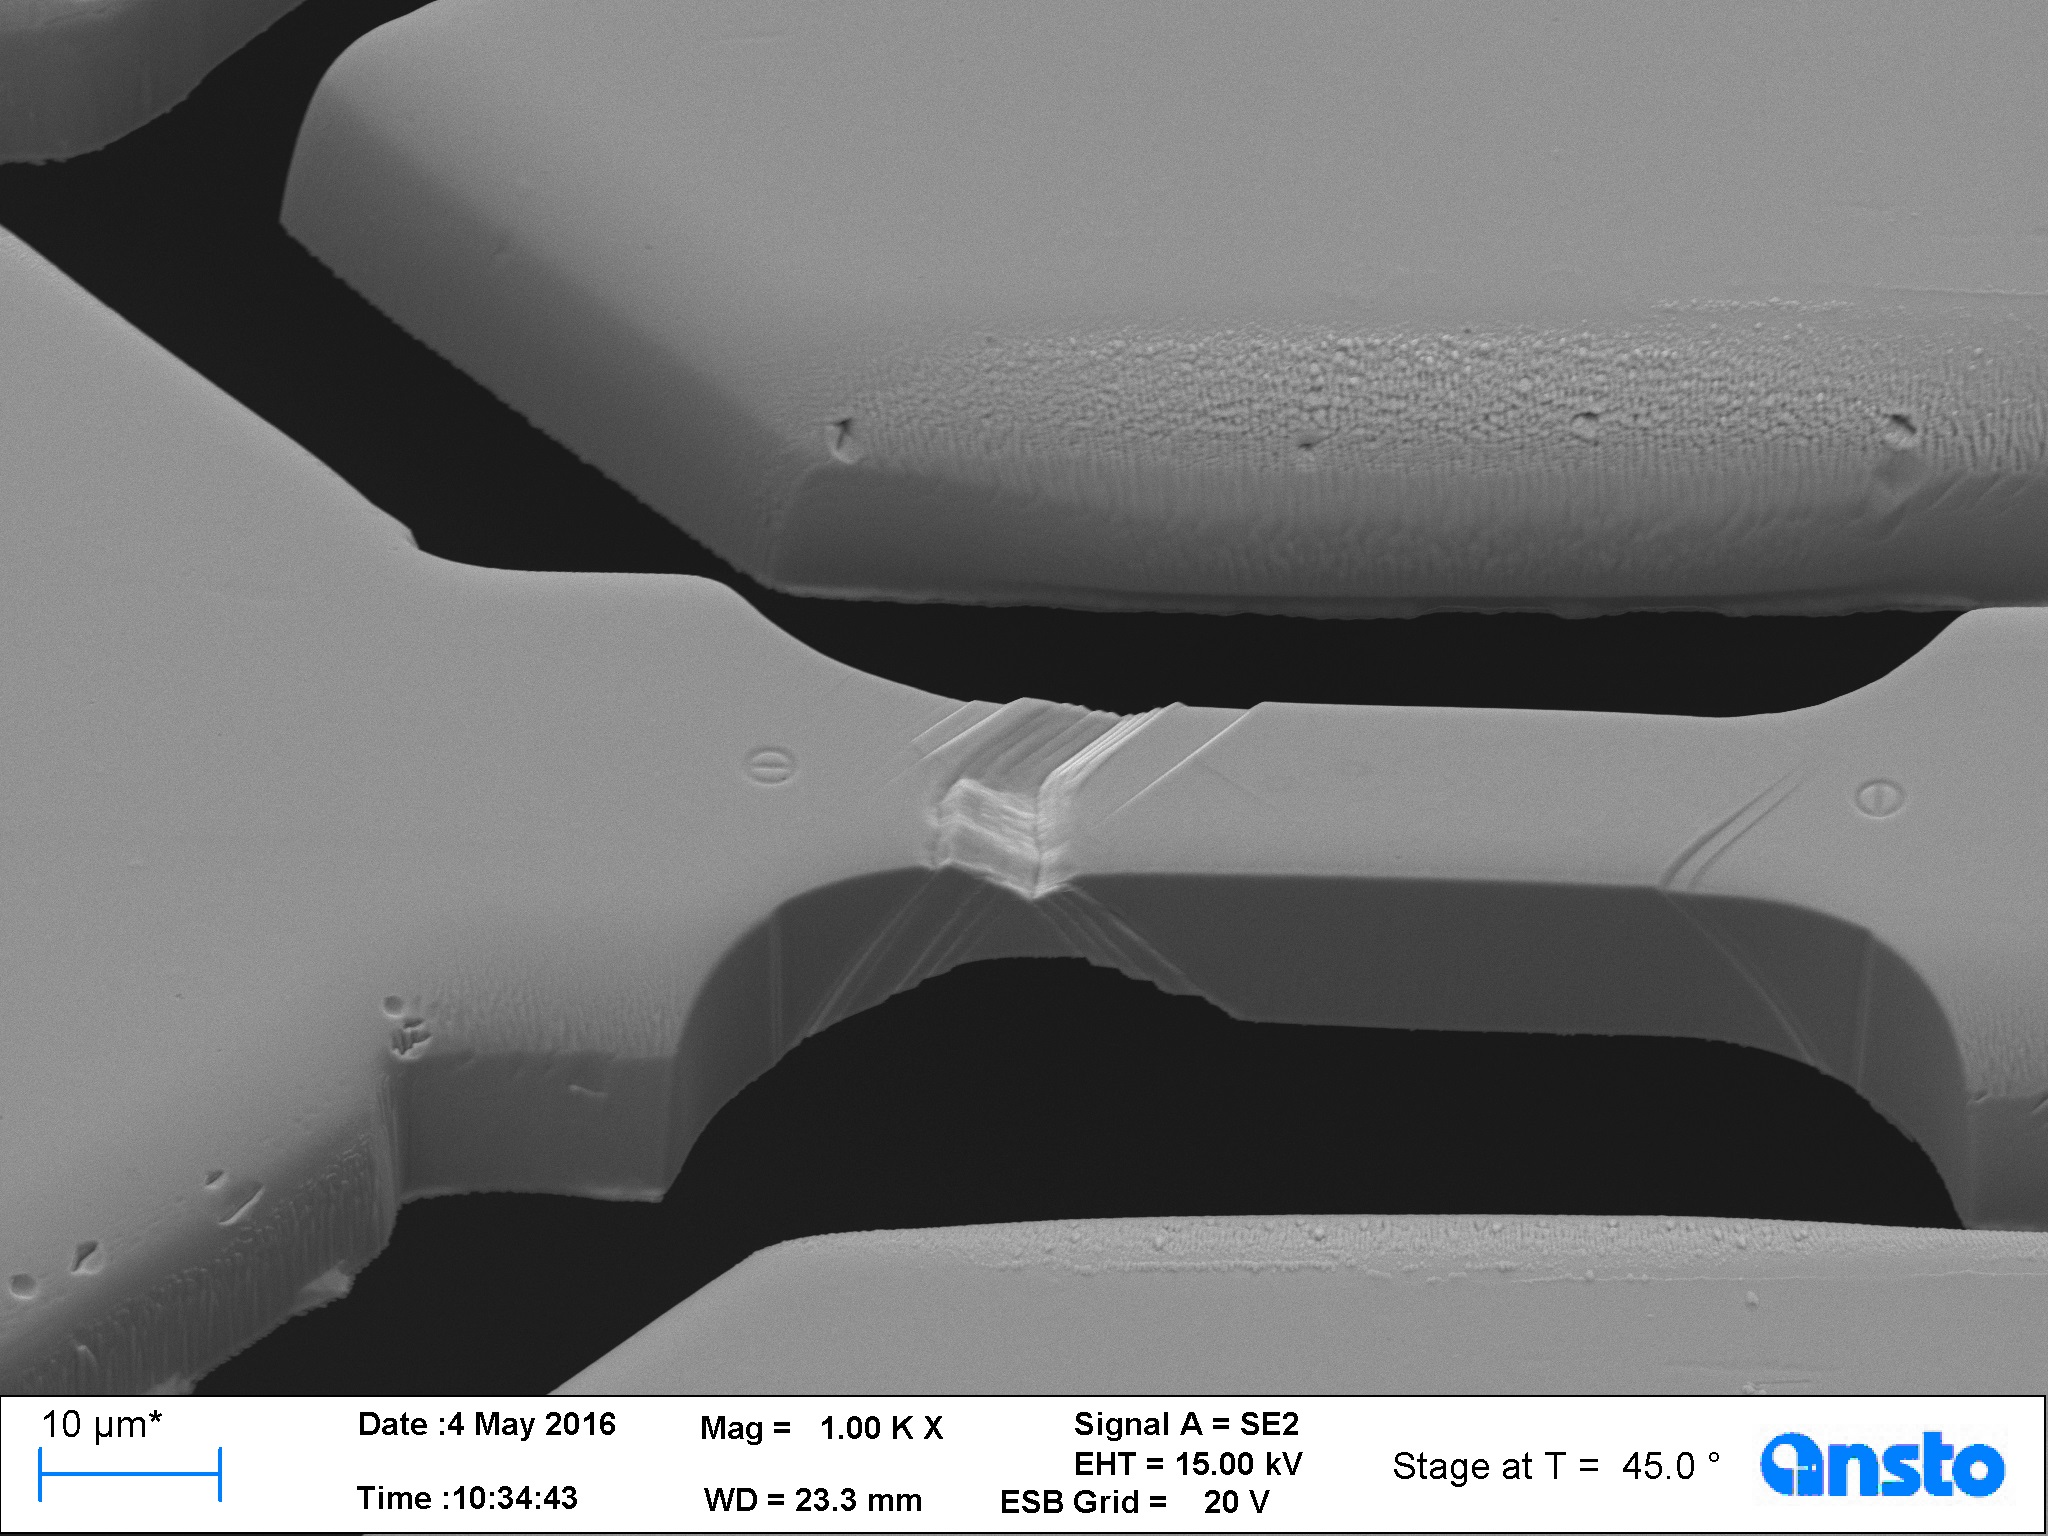
\includegraphics[width=\linewidth]{../data/Ni023.jpg}
    \end{subfigure}
    ~
    \begin{subfigure}[t]{0.3\linewidth}
        \centering
        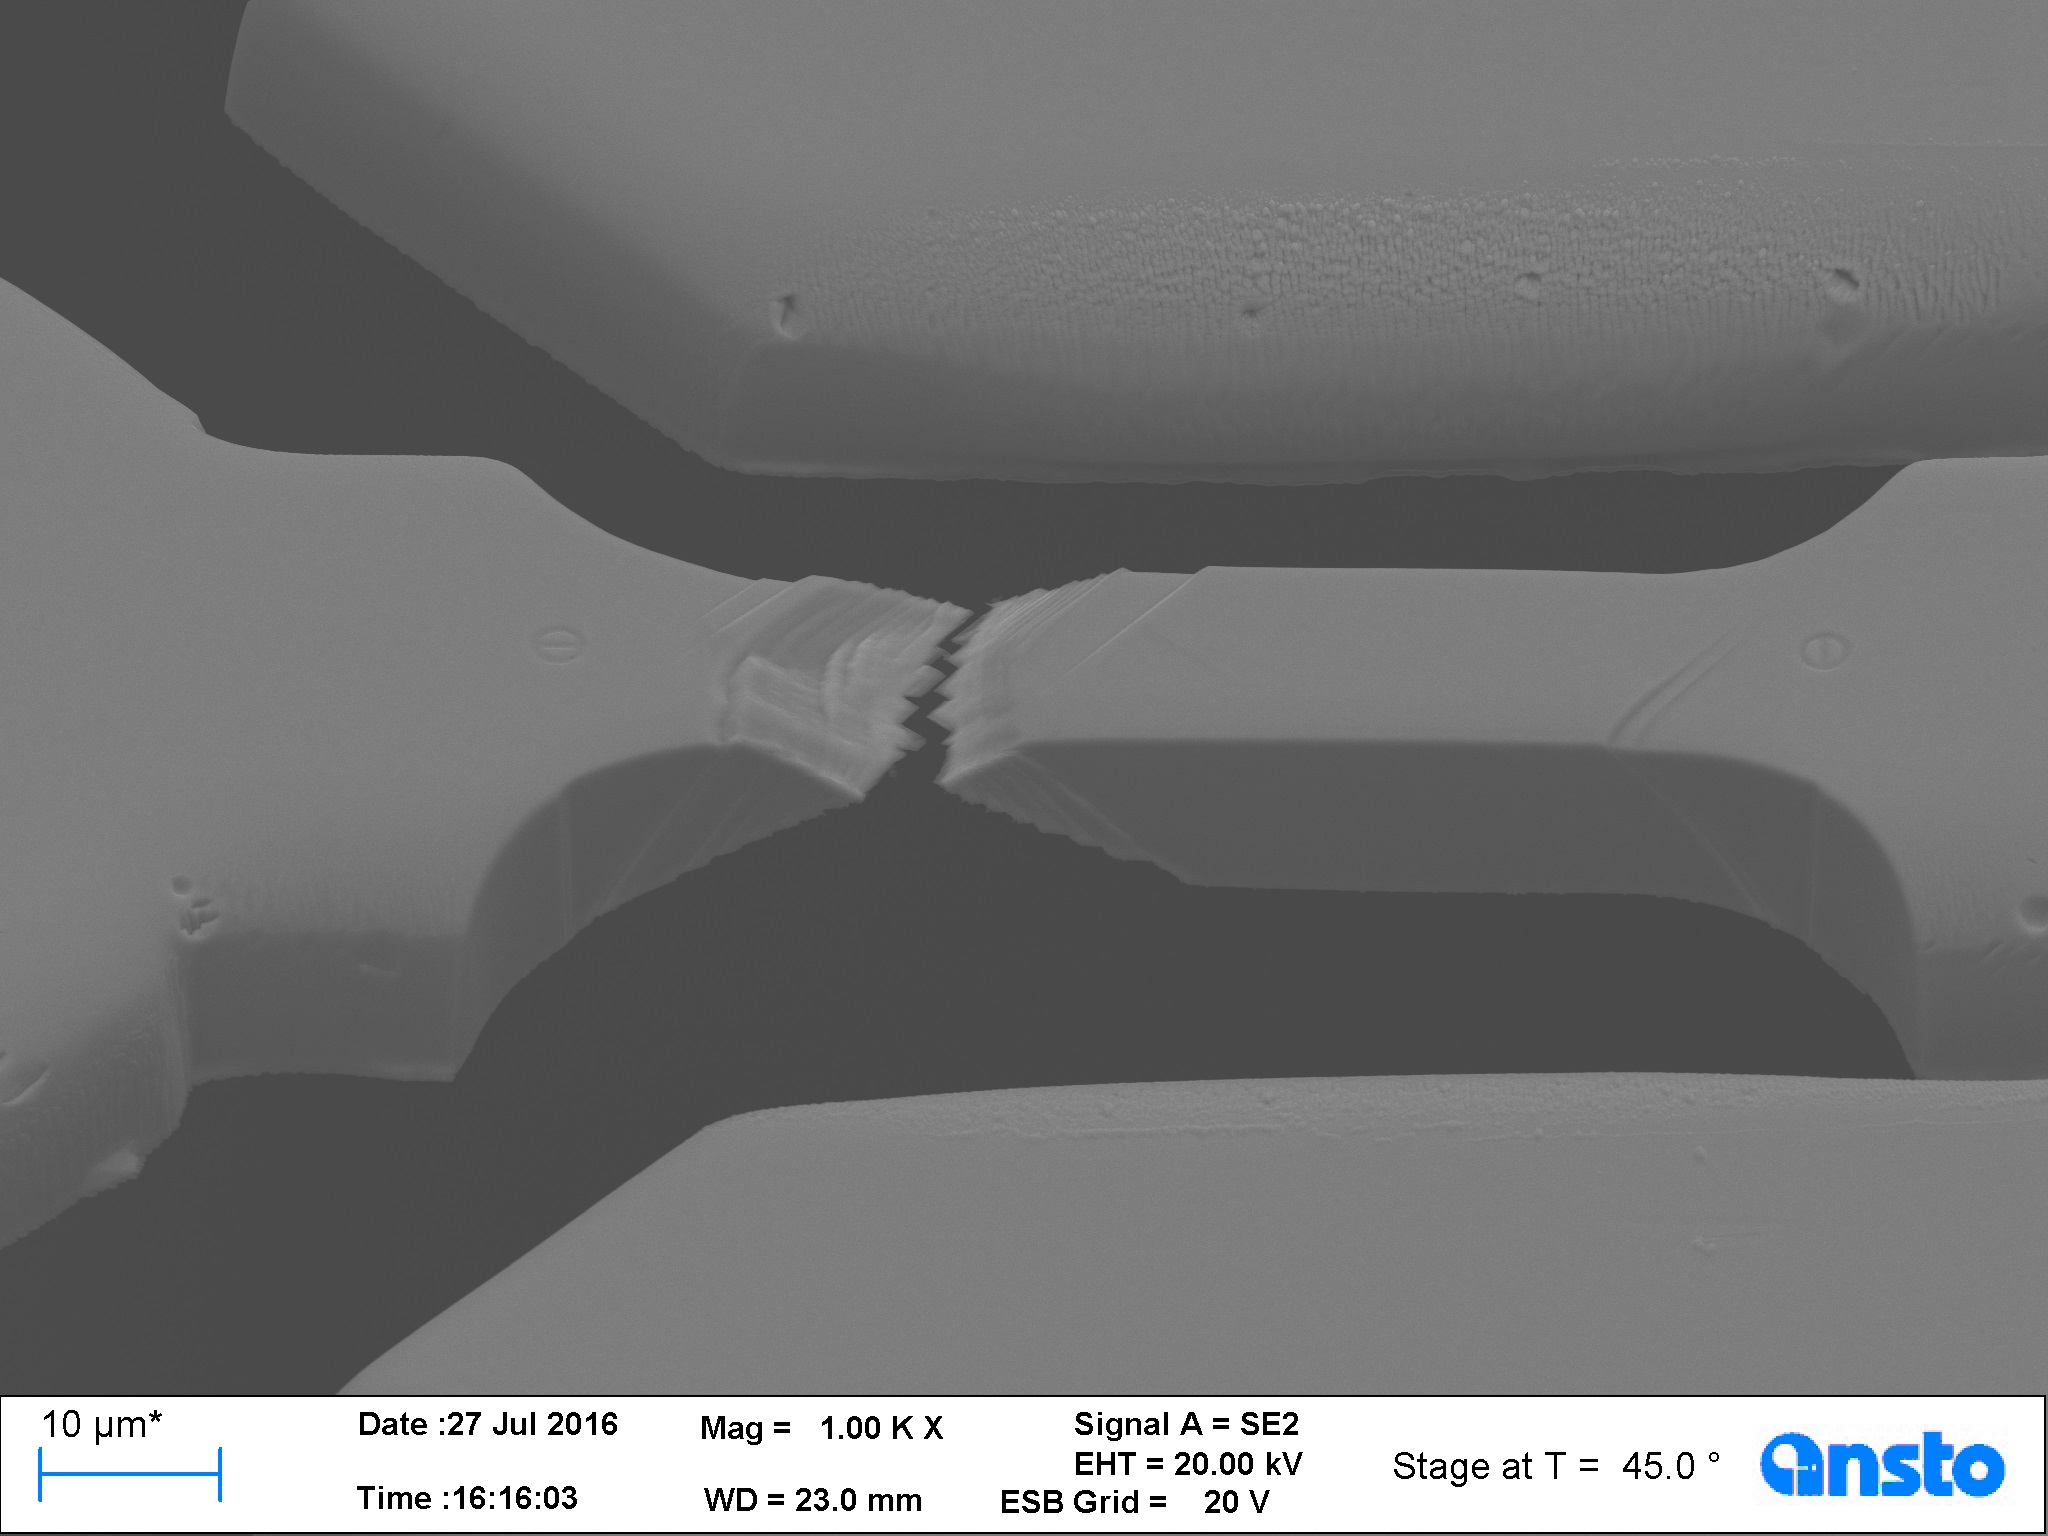
\includegraphics[width=\linewidth]{../data/Ni039.jpg}
    \end{subfigure}
    \caption{Tensile tests taken to failure.}
    \label{f:necking}
\end{figure}

It is worth noting that the timescale of dislocation plasticity simulations make them unsuitable to simulate the entirety of the experiments. EasyDD also does not have the capability to dynamically remesh its finite elements, so it cannot account for fracture. For the same reason, simulation loading rates are higher than experimental ones, we expand on this in \cref{ss:modelSetup}.

\subsection{Dislocation plasticity setup}
\label{ss:modelSetup}

The material parameters of the samples were also not known, so they were estimated from comercially available manufacturing spec sheets and measurements reported from literature. The exact values used for the lattice parameter, shear modulus and Poisson ratio are: $a \coloneqq \SI{3.499}{\angstrom}$, $ \mu  \coloneqq \SI{79e3}{\mega\pascal}$, $\nu \coloneqq 0.31$ respectively. The lattice parameter is from \cite{ni_lattice} and the othters are the mean of the upper and lower values reported by \cite{azom_nickel}.

We used prismatic loops with four sides as Frank-Reed sources to seed the domain with dislocations. Preliminary simulations showed the initially assumed dislocation density was too high, instead it was dropped to a single seed loop per active slip system. For the $\langle 1\, 0\, 0 \rangle$ loading direction, this was 8 loops, and for $\langle 1\, 1\, 0 \rangle$ it was only 4; \cref{t:slipSystems} contains the active slip systems for both scenarios.
\begin{table}
    \centering
    \caption{Active slip systems for prismatic loops in the $\langle 1\, 0\, 0 \rangle$ and $\langle 1\, 1\, 0 \rangle$ tensile loading directions.}
    \label{t:slipSystems}
    \begin{tabular}{rcl}
        \toprule
        Loading direction                            & Slip plane    & Burgers vector           \\
        \midrule
        \multirow{8}{*}{$\langle 1\, 0\, 0 \rangle$} & $(1\, 1\, 1)$ & $[1\, \overline{1}\, 0]$ \\
                                                     & $(1\, 1\, 1)$ & $[1\, \overline{1}\, 0]$ \\
                                                     & $(1\, 1\, 1)$ & $[1\, \overline{1}\, 0]$ \\
                                                     & $(1\, 1\, 1)$ & $[1\, \overline{1}\, 0]$ \\
                                                     & $(1\, 1\, 1)$ & $[1\, \overline{1}\, 0]$ \\
                                                     & $(1\, 1\, 1)$ & $[1\, 0\, \overline{1}]$ \\
                                                     & $(1\, 1\, 1)$ & $[1\, 0\, \overline{1}]$ \\
                                                     & $(1\, 1\, 1)$ & $[1\, 0\, \overline{1}]$ \\
        \midrule
        \multirow{4}{*}{$\langle 1\, 1\, 0 \rangle$} & $(1\, 1\, 1)$ & $[1\, \overline{1}\, 0]$ \\
                                                     & $(1\, 1\, 1)$ & $[1\, \overline{1}\, 0]$ \\
                                                     & $(1\, 1\, 1)$ & $[1\, \overline{1}\, 0]$ \\
                                                     & $(1\, 1\, 1)$ & $[1\, 0\, \overline{1}]$ \\
        \bottomrule
    \end{tabular}
\end{table}
To minimise computation expenditure, we only included these active slip systems in our simulations. This obviously does not fully represent reality, but it saves simulations from having to resolve as many collisions and topological operations as would otherwise occur. Regardless of this decision, the simulations still managed to do an unexpectedly great job at quantitatively, and qualitatively reproducing the experimentally measured strain-stress curves as discussed in \cref{sc:NiResults}.

The pillar length was defined as $\SI{36}{\micro\metre}$, or $3\times$ the length of one of the sides of the square cross-section. The extra length acts as a buffer zone for simulating dislocations moving into the bulk, where they pile up. In the simulation, they stick to the end of the cantilever, as per \cref{c:surfRem}. The initial FR sources were random-uniformly distributed within the central $80\%$ of the domain, i.e. $x \in [0.1X, 0.9X]$, where $x$ is a point along dimension $X$. Given the fact that the number of sources was quite low, various distributions were generated until we arrived at one that spanned the whole domain, rather than clustered about a region.

We define surface node sets $\left\{\forall (x, y, z) \in [0,\, 1] \vert S_{xyz} \in \partial \hat{V}\right\}$, where $\hat{V}$ is a unit volume such that $S_{000}$ denotes the node at the origin, $S_{x00}$ the $x$-axis spanning edge at $y,\, z=0$, and $S_{xy0}$ the $xy$-plane at $z=0$. We use these node sets to define our Neuman (displacement) boundary conditions as follows.
\begin{subequations}
    \begin{align}
        S_{0yz},\, S_{0y0},\, S_{0y1},\, S_{00z},\, S_{01z},\, S_{000},\, S_{001},\, S_{010},\, S_{011} & \gets u_x = 0        \\
        S_{01z},\, S_{010},\, S_{011}                                                                   & \gets u_y = 0        \\
        S_{0y0},\, S_{010},\, S_{000}                                                                   & \gets u_z = 0        \\
        S_{1yz},\, S_{1y0},\, S_{1y1},\, S_{10z},\, S_{11z},\, S_{100},\, S_{101},\, S_{110},\, S_{111} & \gets u_x = U > 0\,.
    \end{align}
\end{subequations}
In simple terms, the whole $yz$-plane at $x=0$ (including corner and edge nodes) is fixed at zero displacement in the $x$-direction; the whole $y$-edge at $x,\,z=0$ (including corner nodes) is also fixed at zero displacement in the $z$-direction; the whole $z$-edge at $x = 0\,\, y = 1$ (including corner nodes) is fixed at zero displacement in the $y$-direction; and the whole $yz$-plane (including corner and edge nodes) nodes at $x=1$ have a displacement, $U > 0$, applied in the $x$-direction ($U < 0$ would be a compressive load). All other degrees of freedom are free to move as necessary.

Once mapped to our simulated cuboid geometry, it looks like \cref{f:tensileSetup}.
\begin{figure}
    \centering
    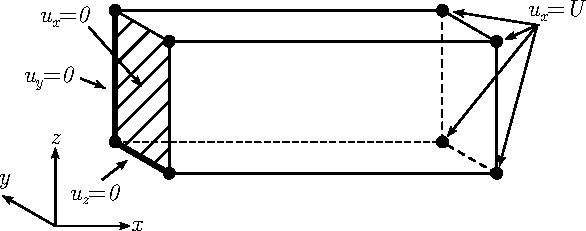
\includegraphics[width=0.8\linewidth]{tensileSetup.pdf}
    \caption[Displacement boundary conditions for dislocation plasticity modelling of single crystal, micro-tensile tests.]{Displacement boundary conditions for dislocation plasticity modelling of single crystal, micro-tensile tests.}
    \label{f:tensileSetup}
\end{figure}

In EasyDD, time is defined in units of shear modulus \cref{eq:timeConversion},
\begin{align}\label{eq:timeConversion}
    t_{\rvar{real}} & = t_{\rvar{sim}} \dfrac{B}{\mu}\,,
\end{align}
where $B \coloneqq 1 \times 10^{-4}[\si{\pascal}][\si{\second}]$ is the dislocation mobility and $\mu \coloneqq [\si{\pascal}]$ is the shear modulus.\footnote{The shear modulus is normalised to 1, we use its magnitude to scale the values of the results accordingly. The edge dislocation mobility is also normalised to 1, other mobilities are defined as multiples of this.}

The experimental loading rates were $\SI{5}{\nano\metre\per\second}$ and $\SI{500}{\nano\metre\per\second}$, which when converted to simulation time, give loading rates that are far too low for the timescales we can simulate. As mentioned in \cref{ss:matrix}, it is important that a quasistatic condition is met for the mobility functions to hold. We therefore chose a loading rate that enabled simulations to advance sufficiently, without overloading the system. We settled on multiplying the converted value\footnote{The converted value used in the simulations is $\left(\SI{5e-3}{\micro\metre}/a\right) \times \left(B /  \mu \right)$, where $a$ is the lattice parameter in micrometers, $B$ the dislocation mobility and $ \mu $ the magnitude of the shear modulus from \cref{eq:timeConversion}.} of the $\SI{5}{\nano\metre\per\second}$ loading rate by a factor of $5 \times 10^6$, which corresponds to a loading rate of $\SI{2.5}{\centi\metre\per\second}$. Any higher and the yield point increased massively, any lower and the simulations took much longer to advance without a significant drop in yield point.

Furthermore, two source segment lengths were trialed. For the $\langle 1\, 0\, 0 \rangle$ loading direction we assumed two values for $\sigma_\rvar{y} = \SI{183, 142}{\mega\pascal}$ and for the $\langle 1\, 1\, 0 \rangle$ direction $\sigma_\rvar{y} = \SI{158, 101}{\mega\pascal}$. The assumptions came from experimental values suggested by Alan and Dhriti and had to be adjusted to account for the simulation higher loading rate. We also did not directly use \cref{eq:yieldStress}, but $l = 2 \mu b / \sigma_\rvar(y)$, to account for the sources being at an angle with respect to the loading direction\footnote{Perhaps it would be more accurate to drop the factor of two and use the critically resolved shear stress instead of the yield stress directly, $\tau = \cos(\phi)\cos(\lambda) \sigma_\rvar{y}$, where $\phi$ and $\lambda$ are the angles between the applied stress, glide plane normal, and glide direction respectively. However, a lot of much stronger assumptions and adjustments had already been made, and this worked satisfactorily.}.

\subsection{Results and discussion}
\label{sc:NiResults}

The experimental measurements go up to fracture, much beyond the domain of dislocation plasticity; they also discard the elastic region, and the early onset of plasticity as shown in \cref{sf:Ni100,sf:Ni110}. Conversely, dislocation plasticity simulations are limited only to small strains, i.e. the part of the curves that typically fall below the experimental limit of detection as shown in \cref{sf:Ni100_DDD,sf:Ni110_DDD}. However, they can elucidate dislocation mechanisms behind plasticity. Here, dislocation plasticity serves as a bridge between the elastic and plastic regimes and lets us explore the mechanisms behind the differences in strain-stress curves between the $\langle 1\,0\,0 \rangle$ and $\langle 1\,1\,0 \rangle$ loading directions.

\begin{figure}
    \centering
    \begin{subfigure}[t]{0.45\linewidth}
        \centering
        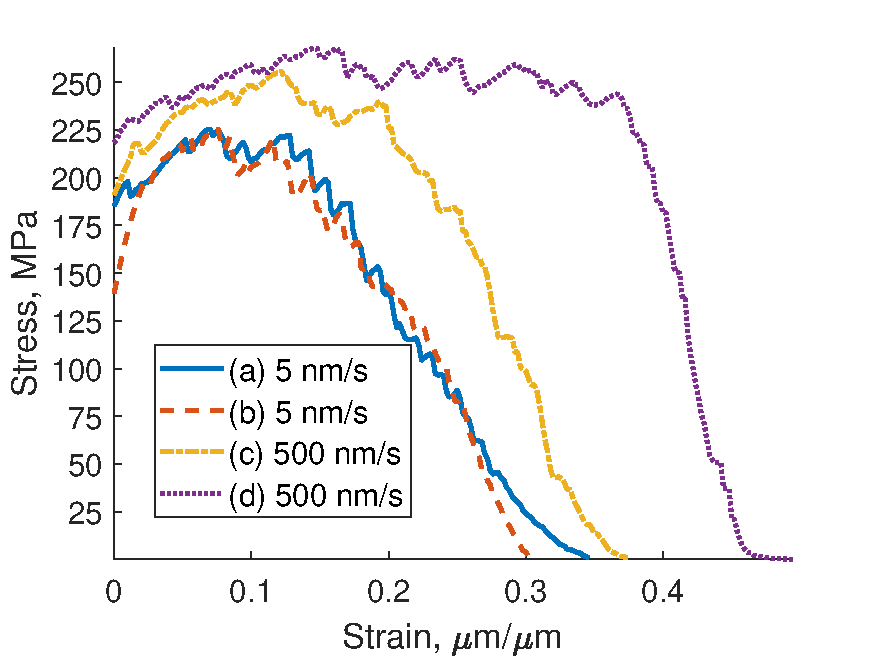
\includegraphics[width=\linewidth]{../data/Ni100.pdf}
        \caption[Tensile loading of Ni in the $\langle 1\, 0\, 0 \rangle$ direction.]{Tensile loading of Ni in the $\langle 1\, 0\, 0 \rangle$ direction.}
        \label{sf:Ni100}
    \end{subfigure}
    ~
    \begin{subfigure}[t]{0.45\linewidth}
        \centering
        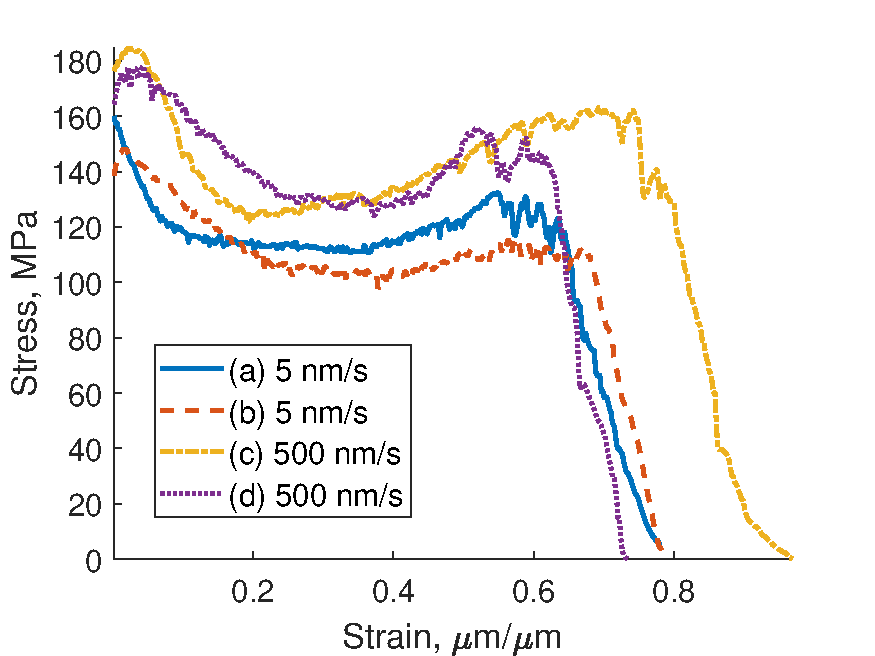
\includegraphics[width=\linewidth]{../data/Ni110.pdf}
        \caption[Tensile loading of Ni in the $\langle 1\, 1\, 0 \rangle$ direction.]{Tensile loading of Ni in the $\langle 1\, 1\, 0 \rangle$ direction.}
        \label{sf:Ni110}
    \end{subfigure}

    \begin{subfigure}[t]{0.45\linewidth}
        \centering
        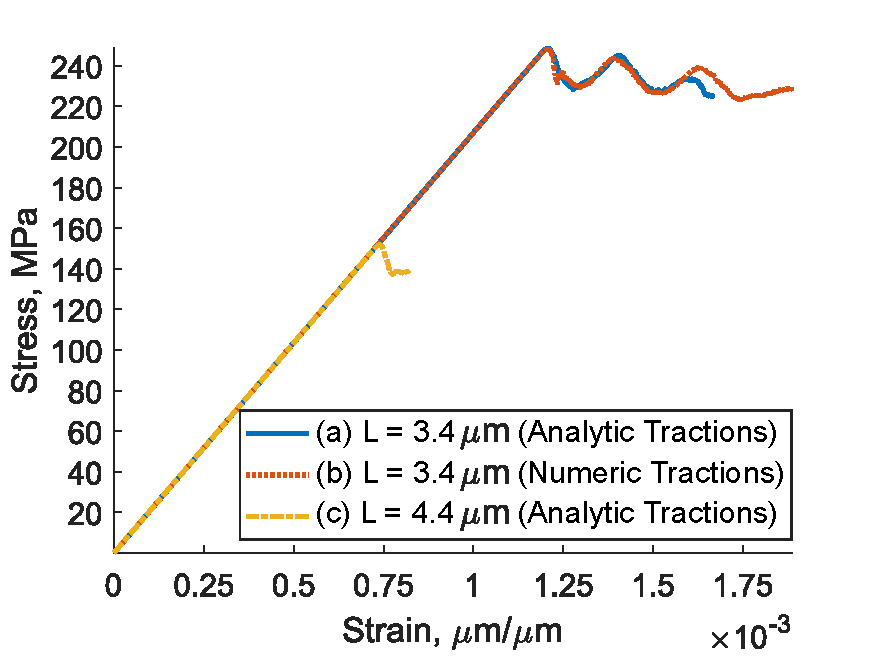
\includegraphics[width=\linewidth]{../data/Ni100_DDD.pdf}
        \caption[Dislocation-Plasticity simulation of tensile loading of Ni in the $\langle 1\, 0\, 0 \rangle$ direction.]{Dislocation-Plasticity simulation of tensile loading of Ni in the $\langle 1\, 0\, 0 \rangle$ direction. (a) and (b) use the same distribution of small sources, (c) uses a different distribution of larger ones. (a) uses analytic tractions and (b) numeric ones.}
        \label{sf:Ni100_DDD}
    \end{subfigure}
    ~
    \begin{subfigure}[t]{0.45\linewidth}
        \centering
        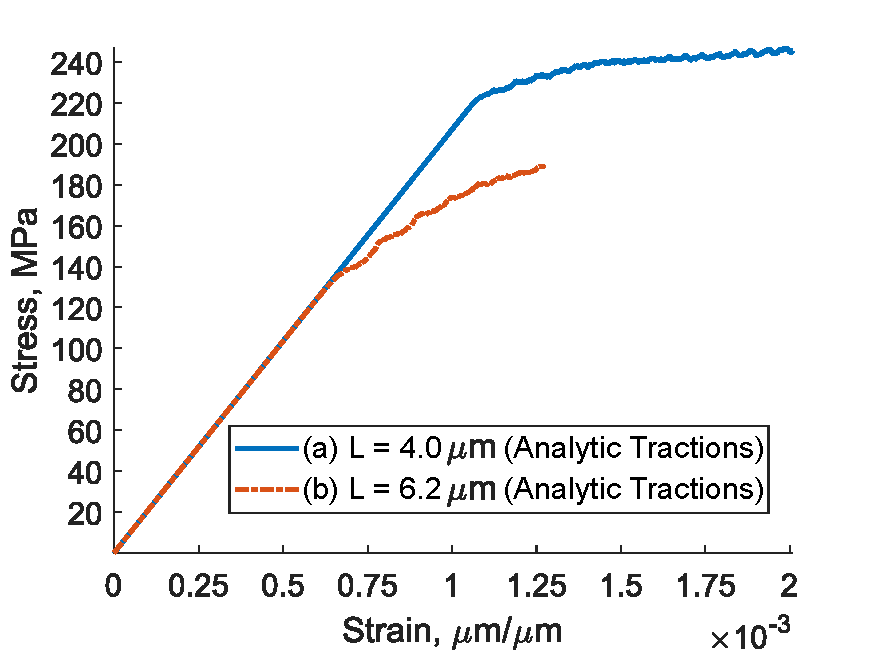
\includegraphics[width=\linewidth]{../data/Ni110_DDD.pdf}
        \caption[Dislocation-Plasticity simulation of tensile loading of Ni in the $\langle 1\, 1\, 0 \rangle$ direction.]{Dislocation-Plasticity simulation of tensile loading of Ni  in the $\langle 1\, 1\, 0 \rangle$ direction. (a) uses small sources, (b) uses a different distribution of larger ones.}
        \label{sf:Ni110_DDD}
    \end{subfigure}
    \caption{Experimental and simulated strain-stress curves of Ni micropillar tensile tests.}
    \label{f:NiStrainStress}
\end{figure}

\Cref{sf:Ni100,sf:Ni110} show the experimental strain stress curves for the $\langle 1\,0\,0 \rangle$ and $\langle 1\,1\,0 \rangle$, respecively. As expected, higher loading rates mean higher stresses overall, and different loading directions produce very different graphs. However, there is quite a large variation between samples even within similar loading rates. This points at dislocations having quite a large effect on the outcome of the experiment. The difference in shape between graphs of both loading directions also point to different slip systems activating at different points and behaving quite differently from each other.

Looking at the low displacement rate curves, (a) and (b) in \cref{sf:Ni100}, it is evident both are quite similar for most of their domain. However, one of the samples yields close to $\SI{140}{\mega\pascal}$ and fails at $30\%$ strain, while the other yields at around $\SI{180}{\mega\pascal}$ and fails closer to $35\%$. These are not insignificant differences, especially at small scales. However, the bulk of the curves look quite similar to one another, and very different to the higher loading rate curves.

Conversely, the high loading rate curves in, (c) and (d) in \cref{sf:Ni100}, are very different to one another. Curve (c) yields at approximately the same point as (a), and the difference in its failure strain and that of curve (a) is less than the difference between curves (a) and (b). That said, curves (c) and (d) are subjected to higher stresses and fail at higher strains than (a) and (b).

\begin{figure}
    \centering
    \begin{subfigure}[t]{0.45\linewidth}
        \centering
        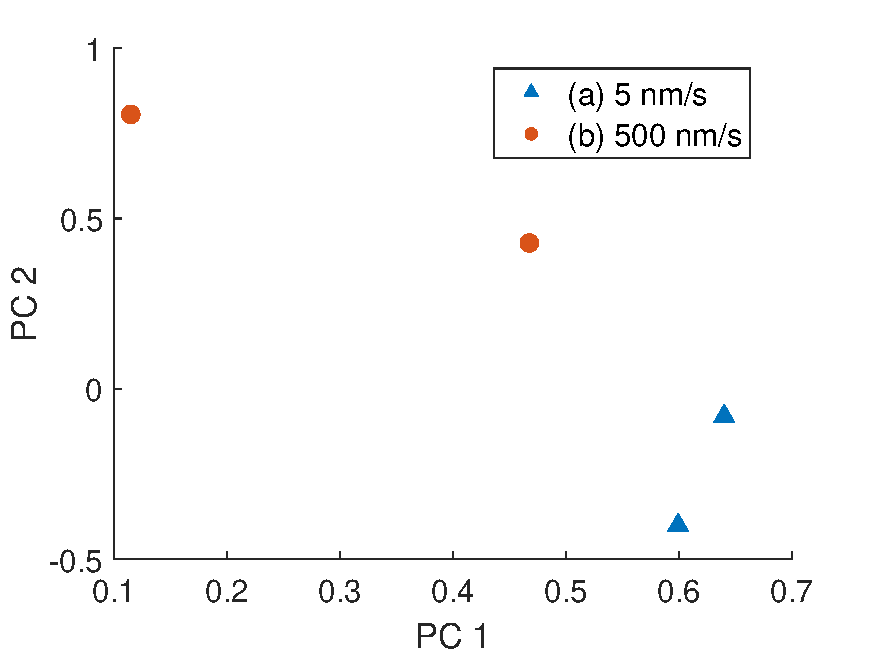
\includegraphics[width=\linewidth]{../data/Ni100_pca.pdf}
        \caption[First two principal components of the Ni strain-stress curves in the $\langle 1\,0\,0 \rangle$ loading direction.]{First two principal components of the Ni strain-stress curves in the $\langle 1\,0\,0 \rangle$ loading direction. First and second principal components respecitvely correspond to $79.41\%$ and $19.05\%$ of the observed variance between curves.}
        \label{sf:Ni100_pca}
    \end{subfigure}
    ~
    \begin{subfigure}[t]{0.45\linewidth}
        \centering
        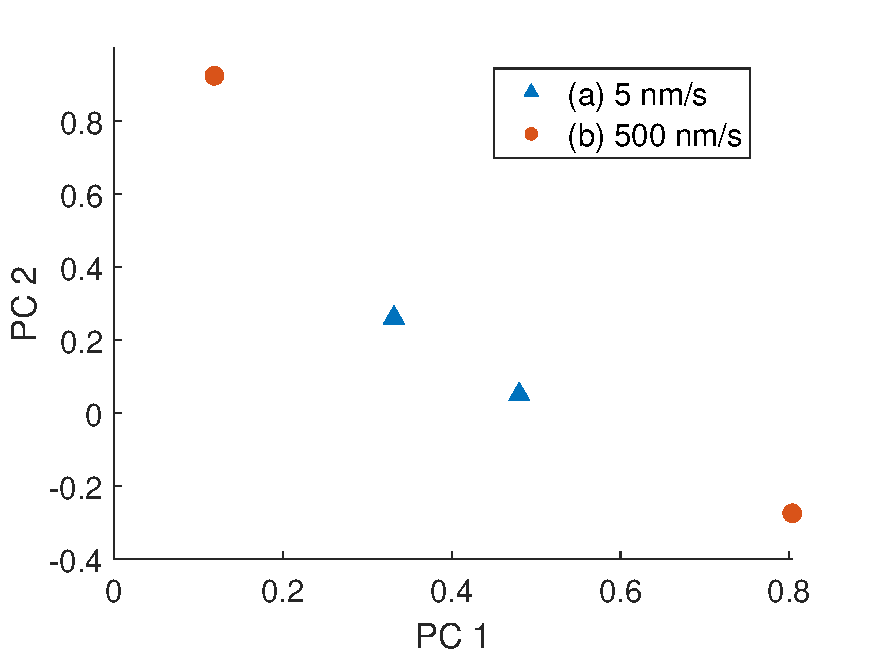
\includegraphics[width=\linewidth]{../data/Ni110_pca.pdf}
        \caption[First two principal components of the Ni strain-stress curves in the $\langle 1\,1\,0 \rangle$ loading direction.]{First two principal components of the Ni strain-stress curves in the $\langle 1\,1\,0 \rangle$ loading direction. First and second principal components respecitvely correspond to $70.61\%$ and $26.21\%$ of the observed variance between curves.}
        \label{sf:Ni110_pca}
    \end{subfigure}
    \caption{Blue triangles (\textcolor{matlabBlue}{$\blacktriangle$}) correspond to the $\SI{5}{\nano\metre\per\second}$ loading rate, orange circles (\textcolor{matlabOrange}{$\bullet$}) that of $\SI{500}{\nano\metre\per\second}$.}
    \label{f:Ni_pca}
\end{figure}

Unfortunately, dislocation plasticity simulations cannot probe such high strains and low loading rates, but it would be interesting to investigate the dislocation mechanisms behind this increased plasticity. One has to wonder whether this is a result of kinetic processes that are typically ignored in dislocation dynamics. However, it may also be the fact that the number of samples is quite limited, so the differences may be due to heterogeneity between samples.

Sadly, sophisticated statistical analyses cannot be performed due to the low number of samples, but we can at least perform a principal component analysis (PCA) and plot the dominant components, as shown in \cref{sf:Ni100_pca}, to see whether the differences between low and high loading rates---respectively denoted by blue triangles (\textcolor{matlabBlue}{$\blacktriangle$}) and orange circles (\textcolor{matlabOrange}{$\bullet$})---are significant. With so few data points, a clustering analysis would not yield quality information.

As expected, the low loading rate measurements cluster together, hinting at similar behaviour. Moreover, the higher loading rates have a larger spread. The Eucledian distance from one of them is even smaller to both low loading rate measurements, than it is to its high loading rate counterpart. More measurements are needed to draw conclusions as to why this is the case. Regardless, it is relatively safe to assume the loading rate has a noticeable effect when loading the $\langle 1\, 0\, 0 \rangle$ direction for these specific rates. Such information is relevant for our simulations, as their loading rates were much higher than these, so we must expect those curves to behave accordingly, and our conclusions must be extrapolated with this in mind.

The story is much different for the $\langle 1\, 1\, 0 \rangle$ loading direction. All graphs in \cref{sf:Ni110} look quite similar. They are markedly different to those in \cref{sf:Ni100}, but among themselves there do not seem to be large differences between low loading rate curves, (a) and (b), and high loading rate ones, (c) and (d). Having said that, curves (c) and (d) consistently experience higher stresses than (a) and (b). With so few samples, it is hard to say whether there is a notable difference.

\Cref{sf:Ni110_pca} confirms this, the Eucledian distance between both low loading rate curves (\textcolor{matlabBlue}{$\blacktriangle$}) is much smaller to one another than that between both high loading rate curves (\textcolor{matlabOrange}{$\bullet$}). With only two data points for each measurement, it is very difficult to assert whether there is a relationship between the first and second principal components that can be used to correlate a curve to its loading rate. We therefore cannot draw satisfacotry conclusions whether such differences in loading rate have much of an effect. Conventional wisdom is that it will, but we cannot quantify how much, so we must tread with care.

Given the computational expense of simulations we cannot perform a meaningful PCA and compare the results to the experimental measurements as we do not have enough samples, and their maximal strains are well below the experimentally measured ones.

Qualitatively and quantitatively, the simulations do a surprisingly good job at reproducing the experimental strain-stress curves. Comparing the yield points and features of \cref{sf:Ni100,sf:Ni110} tith those of \cref{sf:Ni100_DDD,sf:Ni110_DDD} shows remarkable agreement between them. While the simulations cannot reach the same strains as the experiments, they appear to fall within experimental variation, excepting curve (a) of \cref{sf:Ni110_DDD}.

That said, we must be aware that the loading rate is 5 million times higher than $\SI{5}{\nano\meter\per\second}$. As previously mentioned, this loading rate was arrived at by finding the highest loading rate that would not exponentially increase the yield point. However, this does not mean lower loading rates do not decrease the yield point, they do, just not very drastically. They are also impractically slow for our needs.

It is also interesting to note that this was achieved with a very small number of initial sources, only one per active slip system. Contrary to the originally assumed 10 dislocations per square micron. They were also all uniform in size, shape and are all prismatic. These are not wholly unreasonable assumptions, but they are definitely not strictly true. And yet, they did a remarkable job.

\subsection{Conclusions}



% 1929


% TODO